HPCToolkit can measure both the CPU and GPU performance of GPU-accelerated applications. It can measure CPU performance using asynchronous sampling triggered by Linux timers or hardware counter events as described in 
Section~\ref{sample-sources} and it can monitor GPU performance using tool support libraries provided by GPU vendors.

In the following sections, we describe a generic substrate in HPCToolkit to interact with vendor specific runtime systems and libraries and the vendor specific details for measuring performance for NVIDIA, AMD, and Intel GPUs. 

\begin{comment}

To measure both CUDA and OpenMP offloading performance, use one of the CUDA events specified above.
Postprocessing GPU Performance Measurements with HPCToolkit

Collecting Program Structure Information Using Binary Analysis
hpcstruct <load module>
Perform binary analysis to recover program structure of your executable or a shared library, as well as any NVIDIA CUBIN GPU binaries that are embedded in ELF segments. (Clang directly embeds NVIDIA CUBINs in ELF segments.)
hpcstruct hpctoolkit-<your application>-measurements
\end{comment}

\section{Generic Performance Measurement Substrate}

The foundation of HPCToolkit's support for measuring the performance of GPU-accelerated applications is a vendor-independent monitoring substrate. A thin software layer connects NVIDIA's CUPTI (CUDA Performance Tools Interface)~\cite{cupti} and AMD's ROC-tracer (ROCm Tracer Callback/Activity Library)~\cite{roctracer} monitoring libraries to this substrate. The substrate also includes function wrappers to intercept calls to the OpenCL API and Intel's Level 0 API to measure GPU performance for programming models that do not have an integrated measurement substrate 
such as CUPTI or ROC-tracer. 
HPCToolkit reports GPU performance metrics in a vendor-neutral way. For instance, rather than focusing on NVIDIA warps or AMD wavefronts, HPCToolkit presents both as fine-grain, thread-level parallelism.

HPCToolkit supports two levels of performance monitoring for GPU accelerated applications: coarse-grain profiling and tracing of GPU activities at the operation level (e.g., kernel launches, data allocations, memory copies, ...), and fine-grain measurement of GPU computations using PC sampling or instrumentation, which measure GPU computations at the granularity of individual machine instructions.

Coarse-grain profiling attributes to each calling context the total time of all GPU operations initiated in that context. Table~\ref{table:gtimes} shows the classes of GPU operations for which timings are collected. In addition, HPCToolkit records metrics for operations performed including memory allocation and deallocation (Table~\ref{table:gmem}), memory set (Table~\ref{table:gmset}), explicit memory copies (Table~\ref{table:gxcopy}), and synchronization (Table~\ref{table:gsync}). These operation metrics are available for GPUs from all three vendors. 
For NVIDIA GPUs, HPCToolkit also reports GPU kernel characteristics, including including register usage, thread count per block, and theoretical occupancy as shown in Table~\ref{table:gker}. HPCToolkit derives a theoretical GPU occupancy metric as the ratio of the active threads in a streaming multiprocessor to the maximum active threads supported by the hardware in one streaming multiprocessor.

Table~\ref{table:pc-stall} shows fine-grain metrics for GPU instruction execution.
When possible, HPCToolkit attributes fine-grain GPU metrics to both GPU calling contexts and CPU calling contexts.
To our knowledge, no GPU has hardware support for attributing metrics directly to GPU calling contexts.
To compensate, HPCToolkit approximates attributes metrics to GPU calling contexts. It reconstructs GPU calling contexts from static GPU call graphs for 
NVIDIA GPUs (See Section~\label{nvidia-cct}) and uses measurements of call sites and data flow analysis on static call graphs to apportion metrics among call paths in a GPU calling context tree.
We expect to add similar functionality for GPUs from other vendors in the future.

The performance metrics above are reported in a vendor-neutral way. Not every metric is available for all GPUs.
Coarse-grain profiling and tracing are supported for AMD, Intel, and NVIDIA GPUs. HPCToolkit supports fine-grain measurements on NVIDIA GPUs using PC sampling and provides some simple fine-grain measurements on Intel GPUs using instrumentation. 
Currently, AMD GPUs lack both hardware and software support for fine-grain measurement.  The next few sections describe specific measurement capabilities for NVIDIA, AMD, and Intel GPUs, respectively.


\begin{table}[t]
\centering
\begin{tabular}{|l|l|}\hline
Metric & Description\\\hline\hline
 GKER (sec)  &  GPU time: kernel execution (seconds)  \\\hline 
  GMEM (sec)  &  GPU time: memory allocation/deallocation (seconds)  \\\hline 
  GMSET (sec)  &  GPU time: memory set (seconds)  \\\hline 
  GXCOPY (sec)  &  GPU time: explicit data copy (seconds)  \\\hline 
% GICOPY (sec)  &  GPU time: implicit data copy (seconds)  \\\hline 
  GSYNC (sec)  &  GPU time: synchronization (seconds)  \\\hline 
 GPUOP (sec) & Total GPU operation time: sum of all metrics above \\\hline
\end{tabular}
\caption{GPU operation timings.}
\label{table:gtimes}
\end{table}

\begin{table}[t]
\centering
\begin{tabular}{|l|l|}\hline
Metric & Description\\\hline\hline
 GMEM:UNK (B)  &  GPU memory alloc/free: unknown memory kind (bytes)  \\\hline
  GMEM:PAG (B)  &  GPU memory alloc/free: pageable memory (bytes)  \\\hline
  GMEM:PIN (B)  &  GPU memory alloc/free: pinned memory (bytes)  \\\hline
  GMEM:DEV (B)  &  GPU memory alloc/free: device memory (bytes)  \\\hline
  GMEM:ARY (B)  &  GPU memory alloc/free: array memory (bytes)  \\\hline
  GMEM:MAN (B)  &  GPU memory alloc/free: managed memory (bytes)  \\\hline
  GMEM:DST (B)  &  GPU memory alloc/free: device static memory (bytes)  \\\hline
  GMEM:MST (B)  &  GPU memory alloc/free: managed static memory (bytes)  \\\hline
  GMEM:COUNT  &  GPU memory alloc/free: count  \\\hline
\end{tabular}
\caption{GPU memory allocation and deallocation.}
\label{table:gmem}
\end{table}


\begin{table}[t]
\centering
\begin{tabular}{|l|l|}\hline
Metric & Description\\\hline\hline
 GMSET:UNK (B)  &  GPU memory set: unknown memory kind (bytes)  \\\hline
  GMSET:PAG (B)  &  GPU memory set: pageable memory (bytes)  \\\hline
  GMSET:PIN (B)  &  GPU memory set: pinned memory (bytes)  \\\hline
  GMSET:DEV (B)  &  GPU memory set: device memory (bytes)  \\\hline
  GMSET:ARY (B)  &  GPU memory set: array memory (bytes)  \\\hline
  GMSET:MAN (B)  &  GPU memory set: managed memory (bytes)  \\\hline
  GMSET:DST (B)  &  GPU memory set: device static memory (bytes)  \\\hline
  GMSET:MST (B)  &  GPU memory set: managed static memory (bytes)  \\\hline
  GMSET:COUNT  &  GPU memory set: count  \\\hline
\end{tabular}
\caption{GPU memory set metrics.}
\label{table:gmset}
\end{table}

\begin{table}[t]
\centering
\begin{tabular}{|l|l|}\hline
Metric & Description\\\hline\hline
 GXCOPY:UNK (B)  &  GPU explicit memory copy: unknown kind (bytes)  \\\hline 
  GXCOPY:H2D (B)  &  GPU explicit memory copy: host to device (bytes)  \\\hline 
  GXCOPY:D2H (B)  &  GPU explicit memory copy: device to host (bytes)  \\\hline 
  GXCOPY:H2A (B)  &  GPU explicit memory copy: host to array (bytes)  \\\hline 
  GXCOPY:A2H (B)  &  GPU explicit memory copy: array to host (bytes)  \\\hline 
  GXCOPY:A2A (B)  &  GPU explicit memory copy: array to array (bytes)  \\\hline 
  GXCOPY:A2D (B)  &  GPU explicit memory copy: array to device (bytes)  \\\hline 
  GXCOPY:D2A (B)  &  GPU explicit memory copy: device to array (bytes)  \\\hline 
  GXCOPY:D2D (B)  &  GPU explicit memory copy: device to device (bytes)  \\\hline 
  GXCOPY:H2H (B)  &  GPU explicit memory copy: host to host (bytes)  \\\hline 
  GXCOPY:P2P (B)  &  GPU explicit memory copy: peer to peer (bytes)  \\\hline 
  GXCOPY:COUNT  &  GPU explicit memory copy: count  \\\hline 
\end{tabular}
\caption{GPU explicit memory copy metrics.}
\label{table:gxcopy}
\end{table}


\begin{table}[h]
\centering
\begin{tabular}{|l|l|}\hline
Metric & Description\\\hline\hline
 GSYNC:UNK (sec)  &  GPU synchronizations: unknown kind  \\\hline 
  GSYNC:EVT (sec)  &  GPU synchronizations: event  \\\hline 
  GSYNC:STRE (sec)  &  GPU synchronizations: stream event wait  \\\hline 
  GSYNC:STR (sec)  &  GPU synchronizations: stream  \\\hline 
  GSYNC:CTX (sec)  &  GPU synchronizations: context  \\\hline 
  GSYNC:COUNT  &  GPU synchronizations: count  \\\hline 
\end{tabular}
\caption{GPU synchronization metrics.}
\label{table:gsync}
\end{table}


\begin{table}[h]
\centering
\begin{tabular}{|l|l|}\hline
Metric & Description\\\hline\hline
GKER:STMEM (B) & GPU kernel: static memory (bytes)    \\\hline
GKER:DYMEM (B) & GPU kernel: dynamic memory (bytes)   \\\hline
GKER:LMEM (B) & GPU kernel: local memory (bytes)    \\\hline
GKER:FGP\_ACT & GPU kernel: fine-grain parallelism, actual    \\\hline
GKER:FGP\_MAX & GPU kernel: fine-grain parallelism, maximum    \\\hline
GKER:THR\_REG & GPU kernel: thread register count    \\\hline
GKER:BLK\_THR & GPU kernel: thread count   \\\hline
GKER:BLK\_SM (B) & GPU kernel: block local memory (bytes)   \\\hline
GKER:COUNT & GPU kernel: launch count   \\\hline
GKER:OCC\_THR & GPU kernel: theoretical occupancy    \\\hline
\end{tabular}
\caption{GPU kernel characteristic metrics.}
\label{table:gker}
\end{table}

\begin{table}[t]
\centering
\begin{tabular}{|l|p{3.5in}|}\hline
Metric & Description\\\hline\hline
GINST & GPU instructions executed\\\hline
GINST:STL\_ANY  &  GPU instruction stalls: any  \\\hline 
 GINST:STL\_NONE  &  GPU instruction stalls: no stall  \\\hline 
 GINST:STL\_IFET  &  GPU instruction stalls: await availability of next    instruction (fetch or branch delay)  \\\hline 
 GINST:STL\_IDEP  &  GPU instruction stalls: await satisfaction of instruction    input dependence  \\\hline 
 GINST:STL\_GMEM  &  GPU instruction stalls: await completion of global memory    access  \\\hline 
 GINST:STL\_TMEM  &  GPU instruction stalls: texture memory request queue full  \\\hline 
 GINST:STL\_SYNC  &  GPU instruction stalls: await completion of thread or    memory synchronization  \\\hline 
 GINST:STL\_CMEM  &  GPU instruction stalls: await completion of constant or    immediate memory access  \\\hline 
 GINST:STL\_PIPE  &  GPU instruction stalls: await completion of required    compute resources  \\\hline 
 GINST:STL\_MTHR  &  GPU instruction stalls: global memory request queue full  \\\hline 
 GINST:STL\_NSEL  &  GPU instruction stalls: not selected for issue but ready  \\\hline 
 GINST:STL\_OTHR  &  GPU instruction stalls: other  \\\hline 
 GINST:STL\_SLP  &  GPU instruction stalls: sleep  \\\hline 
\end{tabular}
\caption{GPU instruction execution and stall metrics.}
\label{table:pc-stall}
\end{table}

\section{NVIDIA GPUs}

\subsection{Performance Measurement of OpenCL Programs}

\begin{table}[t]
\centering
\begin{tabular}{|l|p{3.5in}|}\hline
Argument to \hpcrun{} & What is monitored\\\hline\hline
{\tt -e gpu=opencl} & coarse-grain profiling of NVIDIA GPU operations using NVIDIA's OpenCL runtime\\\hline
{\tt -e gpu=opencl -t} & coarse-grain profiling and tracing of NVIDIA GPU operations using NVIDIA's OpenCL runtime\\\hline
\end{tabular}
\caption{Monitoring performance on NVIDIA GPUs when using the OpenCL programming model and  NVIDIA's OpenCL runtime.}
\label{nvidia-opencl-monitoring-options} 
\end{table}

When using the OpenCL programming model on NVIDIA GPUs, HPCToolkit supports coarse-grain profiling and tracing of GPU activities.
Supported metrics include GPU operation timings (Table~\ref{table:gtimes}) and a subset of standard metrics for GPU operations such as memory allocation and deallocation (Table~\ref{table:gmem}), memory set (Table~\ref{table:gmset}), explicit memory copies (Table~\ref{table:gxcopy}), and synchronization (Table~\ref{table:gsync})

Table~\ref{nvidia-opencl-monitoring-options} shows the possible command-line arguments to \hpcrun{} for monitoring  OpenCL programs on NVIDIA GPUs. There are two levels of monitoring: profiling, or profiling + tracing. When tracing is enabled,  HPCToolkit will collect a trace of activity for each OpenCL command queue. 

\subsection{Performance Measurement of CUDA Programs}

\begin{table}[t]
\centering
\begin{tabular}{|l|p{3.5in}|}\hline
Argument to \hpcrun{} & What is monitored\\\hline\hline
{\tt -e gpu=nvidia} & coarse-grain profiling of GPU operations\\\hline
{\tt -e gpu=nvidia -t} & coarse-grain profiling and tracing of GPU operations\\\hline
{\tt -e gpu=nvidia,pc} &  coarse-grain profiling of GPU operations; fine-grain profiling og GPU kernels using PC sampling\\\hline
\end{tabular}
\caption{Monitoring performance on NVIDIA GPUs when using NVIDIA's CUDA programming model and runtime.}
\label{nvidia-cuda-monitoring-options} 
\end{table}

When using NVIDIA's CUDA programming model, HPCToolkit supports two levels of performance monitoring for NVIDIA GPUs: coarse-grain profiling and tracing of GPU activities at the operation level, and fine-grain profiling of GPU computations using PC sampling, which measures GPU computations at a granularity of individual machine instructions. Section~\ref{nvidia-pc-sampling} describes fine-grain GPU performance measurement using PC sampling and the metrics it measures or computes. 

While performing coarse-grain GPU monitoring of kernels launches, memory copies, and other GPU activities as a CUDA program executes, HPCToolkit will collect a trace of activity for each GPU stream if tracing is enabled. Table~\ref{nvidia-cuda-monitoring-options} shows the possible command-line arguments to \hpcrun{} that will enable different levels of monitoring  for NVIDIA GPUs for GPU-accelerated code implemented using CUDA. When fine-grain monitoring using PC sampling is enabled, coarse-grain profiling is also performed, so tracing is available in this mode as well. However, since PC sampling dilates the CPU overhead of GPU-accelerated codes, tracing is not recommended when PC sampling is enabled.

Besides the standard metrics for GPU operation timings (Table~\ref{table:gtimes}), memory allocation and deallocation (Table~\ref{table:gmem}), memory set (Table~\ref{table:gmset}), explicit memory copies (Table~\ref{table:gxcopy}), and synchronization (Table~\ref{table:gsync}), HPCToolkit reports GPU kernel characteristics, including including register usage,  thread count per block, and theoretical occupancy as shown in Table~\ref{table:gker}. NVIDIA defines theoretical occupancy as the ratio of the active threads in a streaming multiprocessor to the maximum active threads supported by the hardware in one streaming multiprocessor.





\begin{comment}
\begin{table}
\centering
\begin{tabular}{|l|p{3.5in}|}\hline
Metric & Description\\\hline\hline
 GGMEM:LDC (B)  &  GPU global memory: load cacheable memory (bytes)  \\\hline 
  GGMEM:LDU (B)  &  GPU global memory: load uncacheable memory (bytes)  \\\hline 
  GGMEM:ST (B)  &  GPU global memory: store (bytes)  \\\hline 
  GGMEM:LDC (L2T)  &  GPU global memory: load cacheable (L2 cache transactions)  \\\hline 
  GGMEM:LDU (L2T)  &  GPU global memory: load uncacheable (L2 cache transactions)  \\\hline 
  GGMEM:ST (L2T)  &  GPU global memory: store (L2 cache transactions)  \\\hline 
  GGMEM:LDCT (L2T)  &  GPU global memory: load cacheable    (L2 cache transactions, theoretical)  \\\hline 
  GGMEM:LDUT (L2T)  &  GPU global memory: load uncacheable    (L2 cache transactions, theoretical)  \\\hline 
  GGMEM:STT (L2T)  &  GPU global memory: store    (L2 cache transactions, theoretical)  \\\hline 
\end{tabular}
\caption{GPU global memory metrics.}
\label{table:ggmem}
\end{table}


\begin{table}
\centering
\begin{tabular}{|l|l|}\hline
Metric & Description\\\hline\hline
 GLMEM:LD (B)  &  GPU local memory: load (bytes)  \\\hline 
  GLMEM:ST (B)  &  GPU local memory: store (bytes)  \\\hline 
  GLMEM:LD (T)  &  GPU local memory: load (transactions)  \\\hline 
  GLMEM:ST (T)  &  GPU local memory: store (transactions)  \\\hline 
  GLMEM:LDT (T)  &  GPU local memory: load (transactions, theoretical)  \\\hline 
  GLMEM:STT (T)  &  GPU local memory: store (transactions, theoretical)  \\\hline 
\end{tabular}
\caption{GPU local memory metrics.}
\label{table:gmem}
\end{table}



\begin{table}
\centering
\begin{tabular}{|l|p{3.5in}|}\hline
Metric & Description\\\hline\hline
 GICOPY:UNK (B)  &  GPU implicit copy: unknown kind (bytes)  \\\hline 
  GICOPY:H2D (B)  &  GPU implicit copy: host to device (bytes)  \\\hline 
  GICOPY:D2H (B)  &  GPU implicit copy: device to host (bytes)  \\\hline 
  GICOPY:D2D (B)  &  GPU implicit copy: device to device (bytes)  \\\hline 
  GICOPY:CPU\_PF  &  GPU implicit copy: CPU page faults  \\\hline 
  GICOPY:GPU\_PF  &  GPU implicit copy: GPU page faults  \\\hline 
  GICOPY:THRASH  &  GPU implicit copy: CPU thrashing page faults    (data frequently migrating between processors)  \\\hline 
  GICOPY:THROT  &  GPU implicit copy: throttling    (prevent thrashing by delaying page fault service)  \\\hline 
  GICOPY:RMAP  &  GPU implicit copy: remote maps    (prevent thrashing by pinning memory for a time with    some processor mapping and accessing it remotely)  \\\hline 
  GICOPY:COUNT  &  GPU implicit copy: count  \\\hline 
\end{tabular}
\caption{GPU implicit memory copy metrics.}
\label{table:gtimes}
\end{table}


\begin{table}
\centering
\begin{tabular}{|l|l|}\hline
Metric & Description\\\hline\hline
 GBR:DIV  &  GPU branches: diverged  \\\hline 
  GBR:EXE  &  GPU branches: executed  \\\hline 
\end{tabular}
\caption{GPU branch metrics.}
\label{table:gbr}
\end{table}
\end{comment}


At present, using NVIDIA's CUPTI library adds substantial measurement overhead.  Unlike CPU monitoring based on asynchronous sampling, GPU performance monitoring uses vendor-provided callback interfaces to intercept the initiation of each GPU operation. Accordingly,  the overhead of GPU performance monitoring depends upon how frequently GPU operations are initiated. 
In our experience to date, profiling (and if requested, tracing) on NVIDIA GPUs using NVIDIA's CUPTI interface roughly doubles the execution time of a GPU-accelerated application. In our experience, we have seen NVIDIA's PC sampling dilate the execution time of a GPU-accelerated program by $30\times$ using CUDA 10 or earlier.  Our early experience with CUDA 11 indicates that overhead using PC sampling is much lower and less than $5\times$. The overhead of GPU monitoring is principally on the host side. As measured by CUPTI, the time spent in GPU operations or PC samples is expected to be relatively accurate. However, since execution as a whole is slowed while measuring GPU performance, when evaluating GPU activity reported by HPCToolkit, one must be careful.

For instance, if a GPU-accelerated program runs in 1000 seconds without HPCToolkit monitoring GPU activity but slows to 2000 seconds when GPU profiling and tracing is enabled, then if GPU profiles and traces show that the GPU is active for 25\% of the execution time, one should  re-scale the accurate measurements of GPU activity by considering the $2\times$ dilation when monitoring GPU activity. Without monitoring, one would expect the same level of GPU activity, but the host time would be twice as fast. Thus, without monitoring, the ratio of GPU activity to host activity would be roughly double.
 

\subsection{PC Sampling on NVIDIA GPUs}
\label{nvidia-pc-sampling} 

NVIDIA's GPUs have supported PC sampling since Maxwell~\cite{cuptipcsampling}.
Instruction samples are collected separately on each active streaming
multiprocessor (SM) and merged in a buffer returned by NVIDIA's CUPTI. 
In each sampling period, one warp scheduler of each active SM 
samples the next instruction from one of its active warps. Sampling rotates through
an SM's warp schedulers in a round robin fashion.
When an instruction is sampled, its stall reason (if any) is
recorded. If all warps on a scheduler are stalled when a sample is
taken, the sample is marked as a latency sample, meaning no instruction will be issued by the warp scheduler in the next cycle.
Figure~\ref{fig:pc sampling} shows a PC sampling example on an SM with four schedulers. Among the six collected samples, four are latency samples, so the estimated stall ratio is $4/6$. 

Figure~\ref{table:pc-stall} shows the stall metrics recorded by HPCToolkit using CUPTI's PC sampling. Figure~\ref{table:gsamp} shows PC sampling summary statistics recorded by HPCToolkit. Of particular note is the metric \verb|GSAMP:UTIL|. HPCToolkit computes approximate GPU utilization using information gathered using PC sampling. Given the average clock frequency and the sampling rate, if all SMs are active, then HPCToolkit knows how many instruction samples would be expected ({\tt GSAMP:EXP}) if the GPU was fully active for the interval when it was in use. HPCToolkit approximates the percentage of GPU utilization by comparing the measured samples with the expected samples using the following formula: $100 * {\tt (GSAMP:TOT)/ (GSAMP:EXP)}$.


\begin{figure}[t]
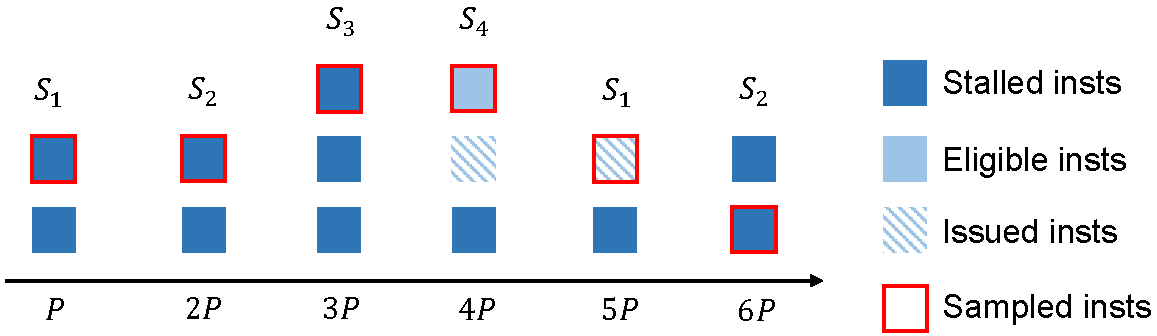
\includegraphics[width=\textwidth]{fig/mental-model.pdf}
\caption{NVIDIA's GPU PC sampling example on an SM. $P-6P$ represent
six sample periods P cycles apart. $S_{1}-S_{4}$ represent four schedulers on an SM.}
\label{fig:pc sampling}
\vspace{-2ex}
\end{figure}

\begin{table}[t]
\centering
\begin{tabular}{|l|l|}\hline
Metric & Description\\\hline\hline
 GSAMP:DRP  &  GPU PC samples: dropped  \\\hline 
  GSAMP:EXP  &  GPU PC samples: expected  \\\hline 
  GSAMP:TOT  &  GPU PC samples: measured  \\\hline 
  GSAMP:PER (cyc)  &  GPU PC samples: period (GPU cycles)  \\\hline 
  GSAMP:UTIL (\%) & GPU utilization computed using PC sampling\\\hline
\end{tabular}
\caption{GPU PC sampling statistics.}
\label{table:gsamp}
\end{table}



For CUDA 10, measurement using PC sampling with CUPTI serializes the execution of GPU kernels. Thus, measurement of GPU kernels using PC sampling will distort the execution of a GPU-accelerated application by blocking concurrent execution of GPU kernels. For applications that rely on concurrent kernel execution to keep the GPU busy, this will significantly distort execution and PC sampling measurements will only reflect the GPU activity of kernels running in isolation.




\subsection{Attributing Measurements to Source Code for NVIDIA GPUs}

NVIDIA's {\tt nvcc} compiler doesn't record information about how GPU machine code maps to CUDA source without proper compiler arguments. Using the {\tt -G} compiler option to {\tt nvcc}, one may generate NVIDIA CUBINs with full DWARF information that includes not only line maps, which map each machine instruction back to a program source line, but also detailed information about inlined code. However, the price of turning on {\tt -G} is that optimization by {\tt nvcc} will be disabled. For that reason, the performance of code compiled {\tt -G} is vastly slower. While a developer of a template-based programming model may find this option useful to see how a program employs templates to instantiate GPU code, measurements of code compiled with {\tt -G} should be viewed with skeptical eye.

One can use {\tt nvcc}'s {\tt -lineinfo } option to instruct {\tt nvcc} to record line map information during compilation.\footnote{Line maps relate each machine instruction back to the program source line from where it came.} The {\tt -lineinfo} option can be used in conjunction with {\tt nvcc} optimization. Using {\tt -lineinfo}, one can measure and interpret the performance of optimized code. However, line map information is a poor substitute for full DWARF information. When {\tt nvcc} inlines code during optimization, the resulting line map information simply shows that source lines that were compiled into a GPU function. A developer examining performance measurements for a function must reason on their own about how any source lines from outside the function got there as the result of inlining and/or macro expansion.

When HPCToolkit uses NVIDIA's CUPTI to monitor a GPU-accelerated application, 
CUPTI notifies HPCToolkit every time it loads a CUDA binary, known as a CUBIN, into a GPU.
At runtime, HPCToolkit computes a cryptographic hash of a CUBIN's contents and records the CUBIN into the execution's measurement directory. 
For instance, if a GPU-accelerated application loaded CUBIN into a GPU, NVIDIA's CUPTI informed HPCToolkit that the CUBIN was being loaded, and HPCToolkit computed its cryptographic hash as {\tt 972349aed8}, then HPCToolkit would record {\tt 972349aed8.gpubin} inside a {\tt gpubins} subdirectory of an HPCToolkit measurement directory.

To  attribute GPU performance measurements back to source, HPCToolkit's \hpcstruct{} supports analysis of NVIDIA CUBIN binaries. Since many CUBIN binaries may be loaded  by a GPU-accelerated application during execution,  an application's measurements directory may contain a {\tt gpubins} subdirectory populated with many CUBINs. In this case, it would be inconvenient to require a developer to apply \hpcstruct{} manually to analyze each CUBIN. To simplify the analysis of an execution's CUBINs, a developer may apply HPCToolkit's \hpcstruct{} directly to a measurement directory to analyze all of the CUBINs it contains. Namely, for a measurements directory {\tt hpctoolkit-laghos-measurements} collected during an execution of the GPU-accelerated laghos mini-app~\cite{laghos}, one can analyze all of the CUBINs collected during execution by using the following command:

\begin{quote}
\begin{verbatim}
hpcstruct hpctoolkit-laghos-measurements
\end{verbatim}
\end{quote}


Since there may be many CUBINs inside an HPCToolkit measurements directory for a GPU-accelerated application, it is useful to accelerate the analysis of an execution's CUBINs by employing parallelism. One can analyze large or many CUBINs in an HPCToolkit measurements directory using multiple threads by specifying \hpcstruct's '\verb|-j|~$n$' option. For instance, one can use 16 threads to analyze the CUBINs in the {\tt hpctoolkit-laghos-measurements} directory with the following command:

\begin{quote}
\begin{verbatim}
hpcstruct -j 16 hpctoolkit-laghos-measurements
\end{verbatim}
\end{quote}

With the default settings of \hpcstruct{}, if the '\verb|-j|~$n$' argument is specified, each CUBIN larger than 100MB will be analyzed using $n$ threads. Smaller CUBINs will be analyzed in parallel by using a pool of $n$ threads to analyze $n$ small CUBINs concurrently. 

By default, when applied to a measurements directory, \hpcstruct{} performs only lightweight analysis of the GPU functions in each CUBIN. When a measurements directory contains fine-grain measurements collected using PC sampling, it is useful to perform a more detailed analysis to recover information about the loops and call sites of GPU functions in an NVIDIA CUBIN. Unfortunately, NVIDIA has refused to provide an API that would enable HPCToolkit to perform instruction-level analysis of CUBINs directly. Instead, HPCToolkit must invoke NVIDIA's {\tt nvdisasm} command line utility to compute control flow graphs for functions in a CUBIN. The version of {\tt nvdisasm} in CUDA 10 is slow and fails to compute control flow graphs for some GPU functions. In such cases, \hpcstruct{} reverts to lightweight analysis of GPU functions that considers only line map information. Because analysis of CUBINs using {\tt nvdisasm} is slow, it is not performed by default. To enable detailed analysis of GPU functions, use the {\tt --gpucfg yes} option to \hpcstruct{}, as shown below:

\begin{quote}
\begin{verbatim}
hpcstruct -j 16 --gpucfg yes hpctoolkit-laghos-measurements
\end{verbatim}
\end{quote}


\subsection{GPU Calling Context Tree Reconstruction}
\label{nvidia-cct}



The CUPTI API returns flat PC samples without any information about GPU call stacks.
With complex code generated from template-based GPU programming models, calling contexts on GPUs are essential for developers to understand the code and its performance. Lawrence Livermore National Laboratory's GPU-accelerated Quicksilver proxy app~\cite{quicksilver} illustrates this problem. Figure~\ref{qs-no-cct} shows a \hpcviewer{} screenshot of Quicksilver without approximate reconstruction the GPU calling context tree. The figure shows a top-down view of heterogeneous calling contexts that span both the CPU and GPU. In the middle of the figure is a placeholder \verb|<gpu kernel>| that is inserted by HPCToolkit. Above the placeholder is a CPU calling context where a GPU kernel was invoked. Below the \verb|<gpu kernel>| placeholder, \hpcviewer{} shows a dozen of the GPU functions that were executed on behalf of the GPU kernel \verb|CycleTrackingKernel|. 

\begin{figure}[t]
\centering
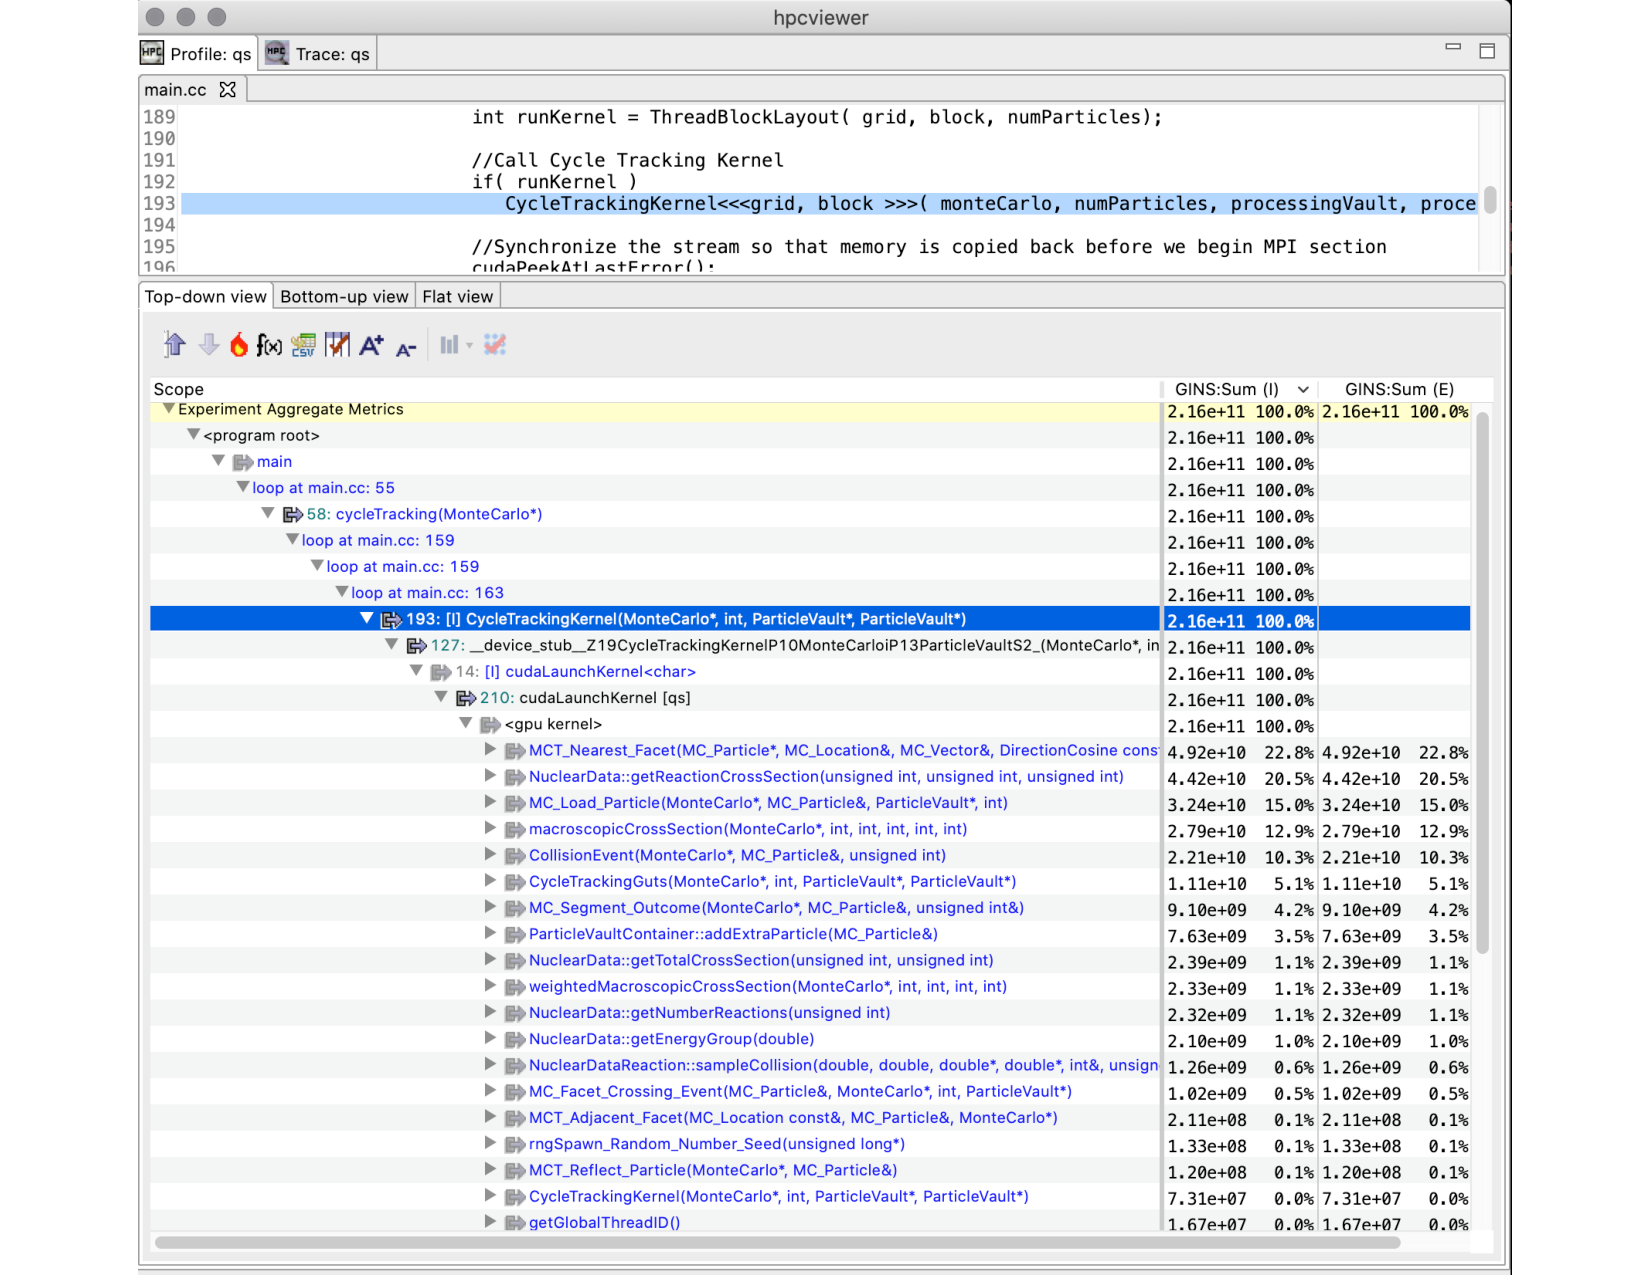
\includegraphics[width=\textwidth]{fig/qs-no-cct.pdf}
\caption{A screenshot of \hpcviewer{} for the GPU-accelerated Quicksilver proxy app without GPU CCT reconstruction.}
\label{qs-no-cct}
\end{figure}


Currently, no API is available for efficiently unwinding call stacks on NVIDIA's GPUs.
To address this issue, we designed a method to reconstruct approximate GPU calling contexts using post-mortem analysis. This analysis is only performed when (1) an execution has been monitored using PC sampling, and (2) an execution's CUBINs have analyzed in detail using \hpcstruct{} with the {\tt --gpucfg yes} option.

To reconstruct approximate calling context trees for GPU computations, HPCToolkit uses information about call sites identified by \hpcstruct{} in conjunction with PC samples measured for each {\tt call} instruction in GPU binaries. 

Without the ability to measure each function invocation in detail, HPCToolkit assumes that each invocation of a particular GPU function incurs the same costs. The costs of each GPU function are apportioned among its caller or callers using the following rules:

\begin{itemize}
\item
If a GPU function G can only be invoked from a single call site, all of the measured cost of G will be attributed to its call site. 
\item
If a GPU function G can be called from multiple call sites and PC samples have been collected for one or more of the call instructions for G, the costs for G are proportionally divided among G's call sites according to the distribution of PC samples for calls that invoke G.  For instance, consider the case where there are three call sites where G may be invoked, 5 samples are recorded for the first call instruction, 10 samples are recorded for the second call instruction, and no samples are recorded for the third call. In this case, HPCToolkit divides the costs for G  among the first two call sites, attributing $5/15$ of G's costs  to the first call site and $10/15$ of G's costs to the second call site. 
\item
If no call instructions for a GPU function G have been sampled, the costs of G are apportioned evenly among each of G's call sites.
\end{itemize}

IHPCToolkit's {\tt hpcprof} analyzes the static call graph associated with each GPU kernel invocation. If the static call graph for the GPU kernel contains cycles, which arise from recursive or mutually-recursive calls,  \hpcprof{} replaces each cycle with a strongly connected component (SCC). In this case, \hpcprof{} unlinks call graph edges between vertices within the SCC and adds an SCC vertex to enclose the set of vertices in each SCC. The rest of \hpcprof{}'s analysis 
treats an SCC vertex as a normal ``function'' in the call graph.

\begin{figure}[t]
\centering
\begin{subfigure}{0.22\textwidth}
\centering
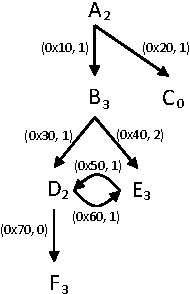
\includegraphics[width=0.6\textwidth]{fig/cct-1.pdf}
\caption{}
\end{subfigure}
~
\begin{subfigure}{0.22\textwidth}
\centering
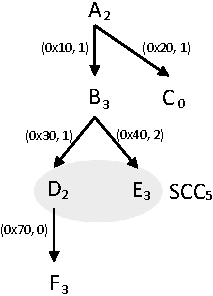
\includegraphics[width=0.6\textwidth]{fig/cct-2.pdf}
\caption{}
\end{subfigure}
~
\begin{subfigure}{0.22\textwidth}
\centering
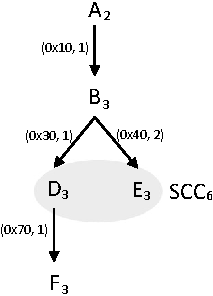
\includegraphics[width=0.6\textwidth]{fig/cct-3.pdf}
\caption{}
\end{subfigure}
~
\begin{subfigure}{0.22\textwidth}
\centering
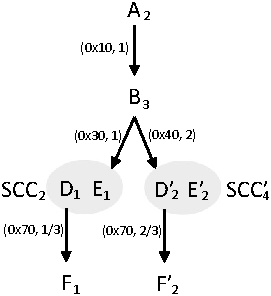
\includegraphics[width=0.8\textwidth]{fig/cct-4.pdf}
\caption{}
\end{subfigure}
\caption{Reconstruct a GPU calling context tree. A-F represent GPU functions. Each subscript denotes the number of samples associated with the function. Each $(a, c)$ pair indicates an edge at address $a$ has $c$ call instruction samples.}
\label{fig:gpu calling context tree}
\end{figure}

\begin{figure}[t]
\centering
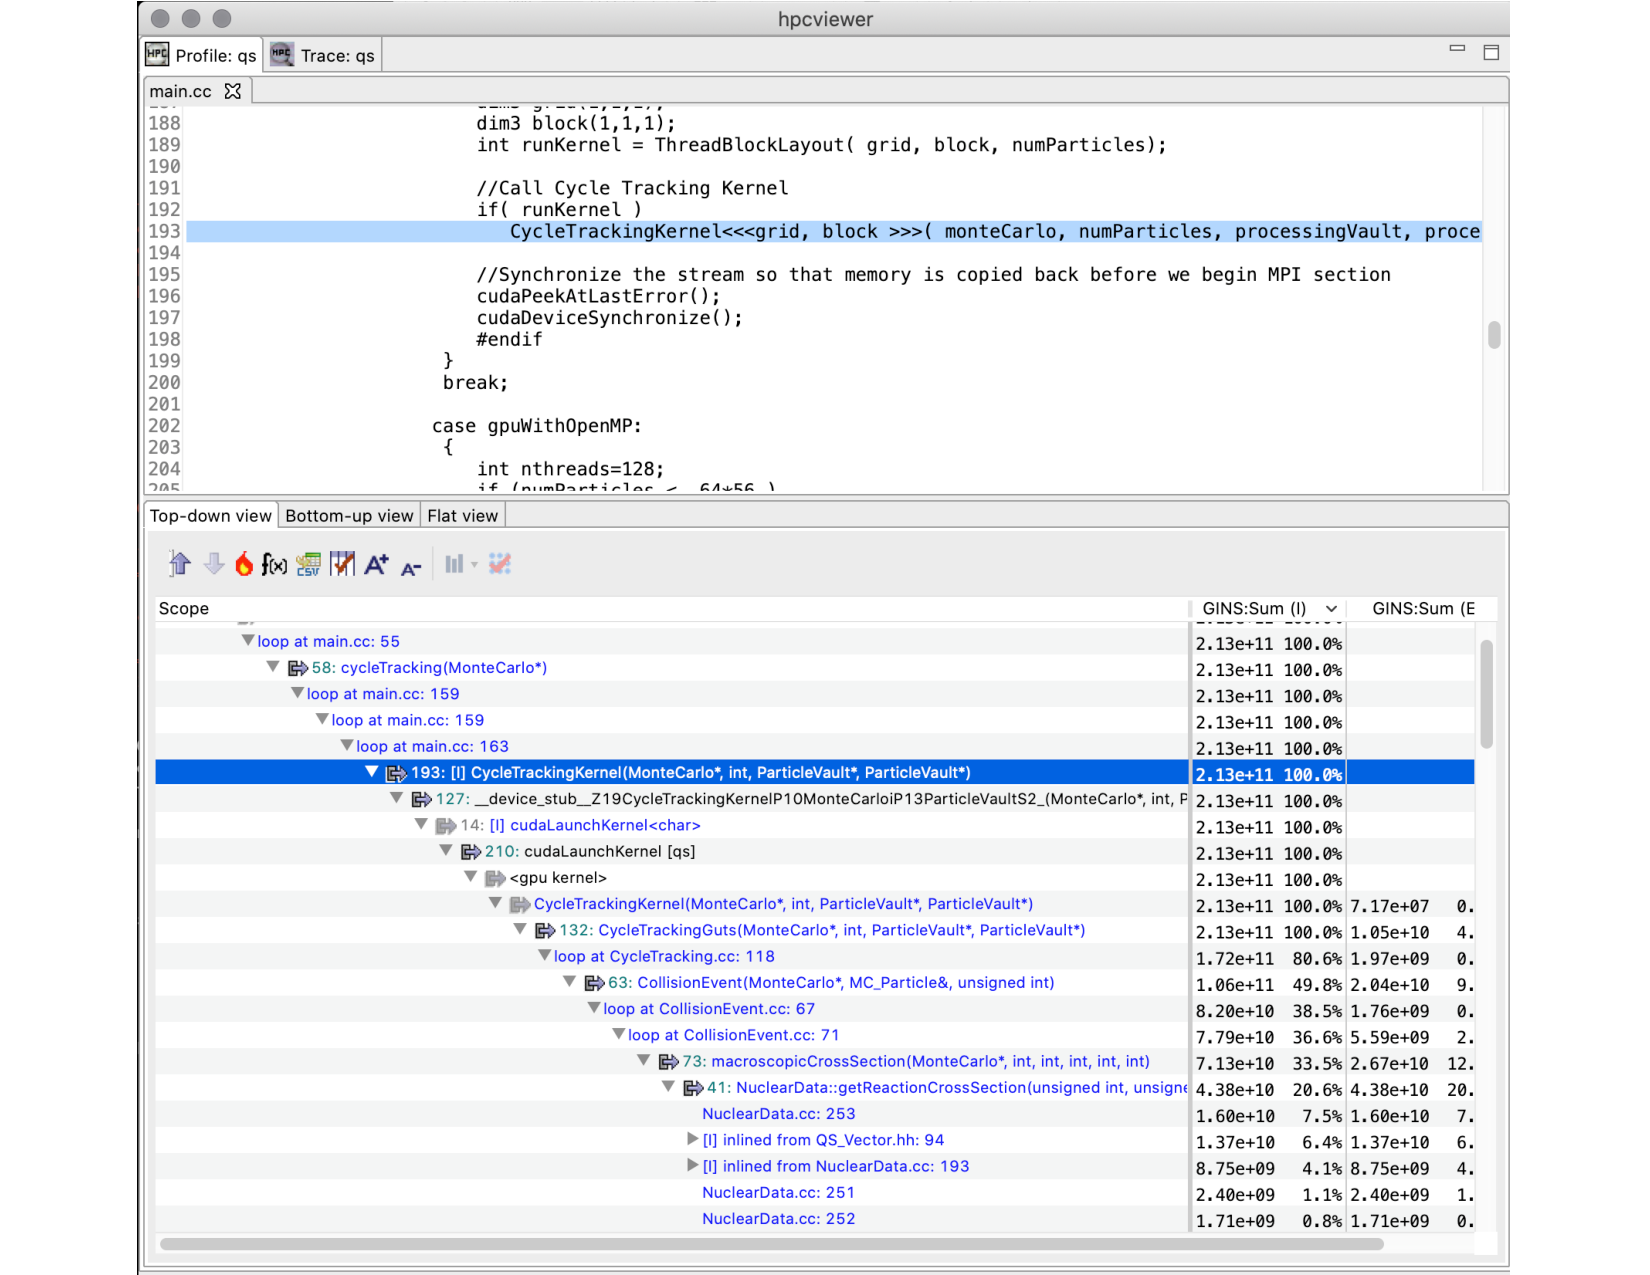
\includegraphics[width=\textwidth]{fig/qs-cct.pdf}
\caption{A screenshot of \hpcviewer{} for the GPU-accelerated Quicksilver proxy app with GPU CCT reconstruction.}
\label{qs-cct}
\end{figure}

Figure~\ref{fig:gpu calling context tree} illustrates the reconstruction of an approximate calling context tree for a GPU computation given the static call graph (computed by \hpcstruct{} from a CUBIN's machine instructions) and PC sample counts for some or all GPU instructions in the CUBIN. Figure~\ref{qs-cct} shows an \hpcviewer{} screenshot for the GPU-accelerated Quicksilver proxy app following reconstruction of GPU calling contexts using the algorithm described in this section. Notice that after the reconstruction, one can see that \verb|CycleTrackingKernel| calls \verb|CycleTrackingGuts|, which calls \verb|CollisionEvent|, which eventually calls  \verb|macroscopicCrossSection| and \verb|NuclearData::getNumberOfReactions|. The the rich  approximate GPU calling context tree reconstructed by \hpcprof{} also shows loop nests and inlined code.\footnote{The control flow graph used to produce this reconstruction for Quicksilver was computed with CUDA 11. You will not be able to reproduce these results with earlier versions of CUDA due to weaknesses in  
{\tt nvdisasm} prior to CUDA 11.}



\section{AMD GPUs}

HPCToolkit supports coarse-grain profiling of GPU-accelerated  applications that offload computation onto AMD GPUs using  AMD's HIP programming model. Table~\ref{amd-options} shows arguments to \hpcrun{} to monitor the performance of GPU operations by HIP programs on AMD GPUs. 
With this coarse-grain profiling support, HPCToolkit can collect GPU operation timings (Table~\ref
{table:gtimes}) and a subset of standard metrics for GPU operations such as memory allocation and deallocation (Table~\ref{table:gmem}), memory set (Table~\ref{table:gmset}), explicit memory copies (Table~\ref{table:gxcopy}), and synchronization (Table~\ref{table:gsync}). 

HPCToolkit also supports coarse-grain profiling of GPU-accelerated OpenCL applications on AMD GPUs. Table~\ref{amd-opencl-options} shows arguments to \hpcrun{} to monitor the performance of OpenCL programs on AMD GPUs. 
As on other GPUs, the OpenCL monitoring interface supports collection of a variety of metrics such as GPU operation timings (Table~\ref{table:gtimes}) 
and a subset of standard metrics for GPU operations such as memory allocation and deallocation (Table~\ref{table:gmem}), memory set (Table~\ref{table:gmset}), explicit memory copies (Table~\ref{table:gxcopy}), and synchronization (Table~\ref{table:gsync})


\begin{table}[t]
\centering
\begin{tabular}{|l|p{3.5in}|}\hline
Argument to \hpcrun{} & What is monitored\\\hline\hline
{\tt -e gpu=amd} & coarse-grain profiling of AMD GPU operations\\\hline
{\tt -e gpu=amd -t} & coarse-grain profiling and tracing of AMD GPU operations\\\hline
\end{tabular}
\caption{Monitoring performance on AMD GPUs when using AMD's HIP programming model and runtime.}
\label{amd-options}
\end{table}


\begin{table}[t]
\centering
\begin{tabular}{|l|p{3.5in}|}\hline
Argument to \hpcrun{} & What is monitored\\\hline\hline
{\tt -e gpu=opencl} & coarse-grain profiling of AMD GPU operations using AMD's OpenCL runtime\\\hline
{\tt -e gpu=opencl -t} & coarse-grain profiling and tracing of AMD GPU operations using AMD's OpenCL runtime\\\hline
\end{tabular}
\caption{Monitoring performance on AMD GPUs when using the OpenCL programming model and AMD's OpenCL runtime.}
\label{amd-opencl-options}
\end{table}


At present, the hardware and software stack for AMD GPUs lacks support for fine-grain (instruction-level) performance measurement of GPU computations.

\section{Intel GPUs}


{
\centering
 \fbox{\parbox{\textwidth}{Note: While HPCToolkit provides initial support for measurement and analysis of GPU-accelerated applications on Intel GPUs,  at the writing of this manual, fine-grain measurement of Intel GPU kernels with GT-Pin only works with non-public versions of Intel's compute runtime. Non-public versions of Intel's GPU compute runtime available in Argonne National Laboratory's Joint Laboratory for Systems Evaluation (JLSE) support fine-grain measurement of GPU kernels with GT-Pin..}}
 \vspace{2ex}
}


\begin{table}[t]
\centering
\begin{tabular}{|l|p{3.5in}|}\hline
Argument to \hpcrun{} & What is monitored\\\hline\hline
{\tt -e gpu=opencl} & coarse-grain profiling of Intel GPU operations using Intel's OpenCL runtime\\\hline
{\tt -e gpu=opencl -t} & coarse-grain profiling and tracing of Intel GPU operations using Intel's OpenCL runtime\\\hline
{\tt -e gpu=opencl,inst} & coarse-grain profiling of Intel GPU operations using Intel's OpenCL runtime;  fine-grain profiling of Intel GPU kernel executions using Intel's GT-Pin \\\hline
\end{tabular}
\caption{Monitoring performance on Intel GPUs when using Intel's OpenCL runtime.}
\label{intel-opencl-options}
\end{table}

%\begin{table}[t]
%\centering
%\begin{tabular}{|l|p{3.5in}|}\hline
%Argument to \hpcrun{} & What is monitored\\\hline\hline
%{\tt -e gpu=level0} & coarse-grain profiling of Intel GPU operations using Intel's Level 0 runtime\\\hline
%{\tt -e gpu=level0 -t} & coarse-grain profiling and tracing of Intel GPU operations using Intel's Level 0 runtime\\\hline
%{\tt -e gpu=level0,inst} & coarse-grain profiling and tracing of Intel GPU operations;  fine-grain profiling of Intel GPU kernel executions using Intel's GT-Pin\\\hline
%\end{tabular}
%\caption{Monitoring performance on Intel GPUs when using Intel's Level 0 runtime.}
%\label{intel-level0-options}
%\end{table}

HPCToolkit supports coarse-grain profiling of GPU-accelerated  applications that offload computation onto Intel GPUs using  OpenCL or Intel's Data-parallel C++ programming model supported by the {\tt dpcpp} compiler. At program launch, a user can select whether Intel's Data-parallel C++ programming model is to execute atop Intel's OpenCL runtime or Intel's Level 0 runtime. For each of these runtimes, HPCToolkit supports both coarse-grain monitoring of GPU operations by intercepting their interface operations.  Table~\ref{intel-opencl-options} shows available options for using HPCToolkit with Intel's OpenCL runtime.
HPCToolkit supports coarse-grain profiling of Intel GPU operations using Intel's Level 0 runtime with argument ``{\tt -e gpu=level0}'' to \hpcrun{}.

With this coarse-grain profiling support, HPCToolkit can collect GPU operation timings (Table~\ref
{table:gtimes}) and a subset of standard metrics for GPU operations such as memory allocation and deallocation (Table~\ref{table:gmem}), memory set (Table~\ref{table:gmset}), explicit memory copies (Table~\ref{table:gxcopy}), and synchronization (Table~\ref{table:gsync}). 


